\section{Quadcopter flight tests}

After validating the performance and safety of the control algorithms in the simulated environment, the next step involves conducting flight tests with a fully-built physical UAV. This final phase of the validation process aims to assess the performance of the developed software with all the previously analysed components together in a real quadcopter during flight. To achieve this, first, the base vehicle will be constructed using the chosen development kit. Subsequently, all additional components required for this project, such as the companion computer and camera, will be integrated into the base frame. Once the vehicle can successfully fly with the full payload under remote control, the developed control solutions will be tested.

The initial test will run the hand-control solution to verify that the autopilot can receive flight commands from an offboard computer outside of the simulation. Next, the follow mechanism will be started to confirm that the companion computer can function in flight as well as it did during the simulation tests.

The exact steps that will be executed one after the other to ensure that safety is maintained during the whole process are as follows:
\begin{enumerate}
    \item Assemble the quadcopter with its basic components.
    \item Attach the custom payload.
    \item Conduct a test flight using only the remote control and factory autopilot while monitoring through QGroundControl.
    \item Perform a flight using the custom software from an offboard computer, utilizing the \texttt{test-camera} tool.
    \item Conduct a flight using the \texttt{test-camera} tool from the onboard computer.
    \item Perform a flight using the custom hand-gesture control solution from the offboard computer.
    \item Conduct a flight using the custom follow solution from the onboard computer.
\end{enumerate}


\subsection{Build process}
\label{sec:test-7-builddrone}

The chosen vehicle for this project is the Holybro X500, specifically designed to be compatible with PX4. The PX4 documentation\footnote{\url{https://docs.px4.io/main/en/frames_multicopter/holybro_x500_pixhawk4.html}} provides detailed instructions on how to build the vehicle using its Development Kit. Figure \ref{fig:x500-dev-kit} illustrates all the components required to construct the complete vehicle.

\begin{figure}[H]
  \centering
  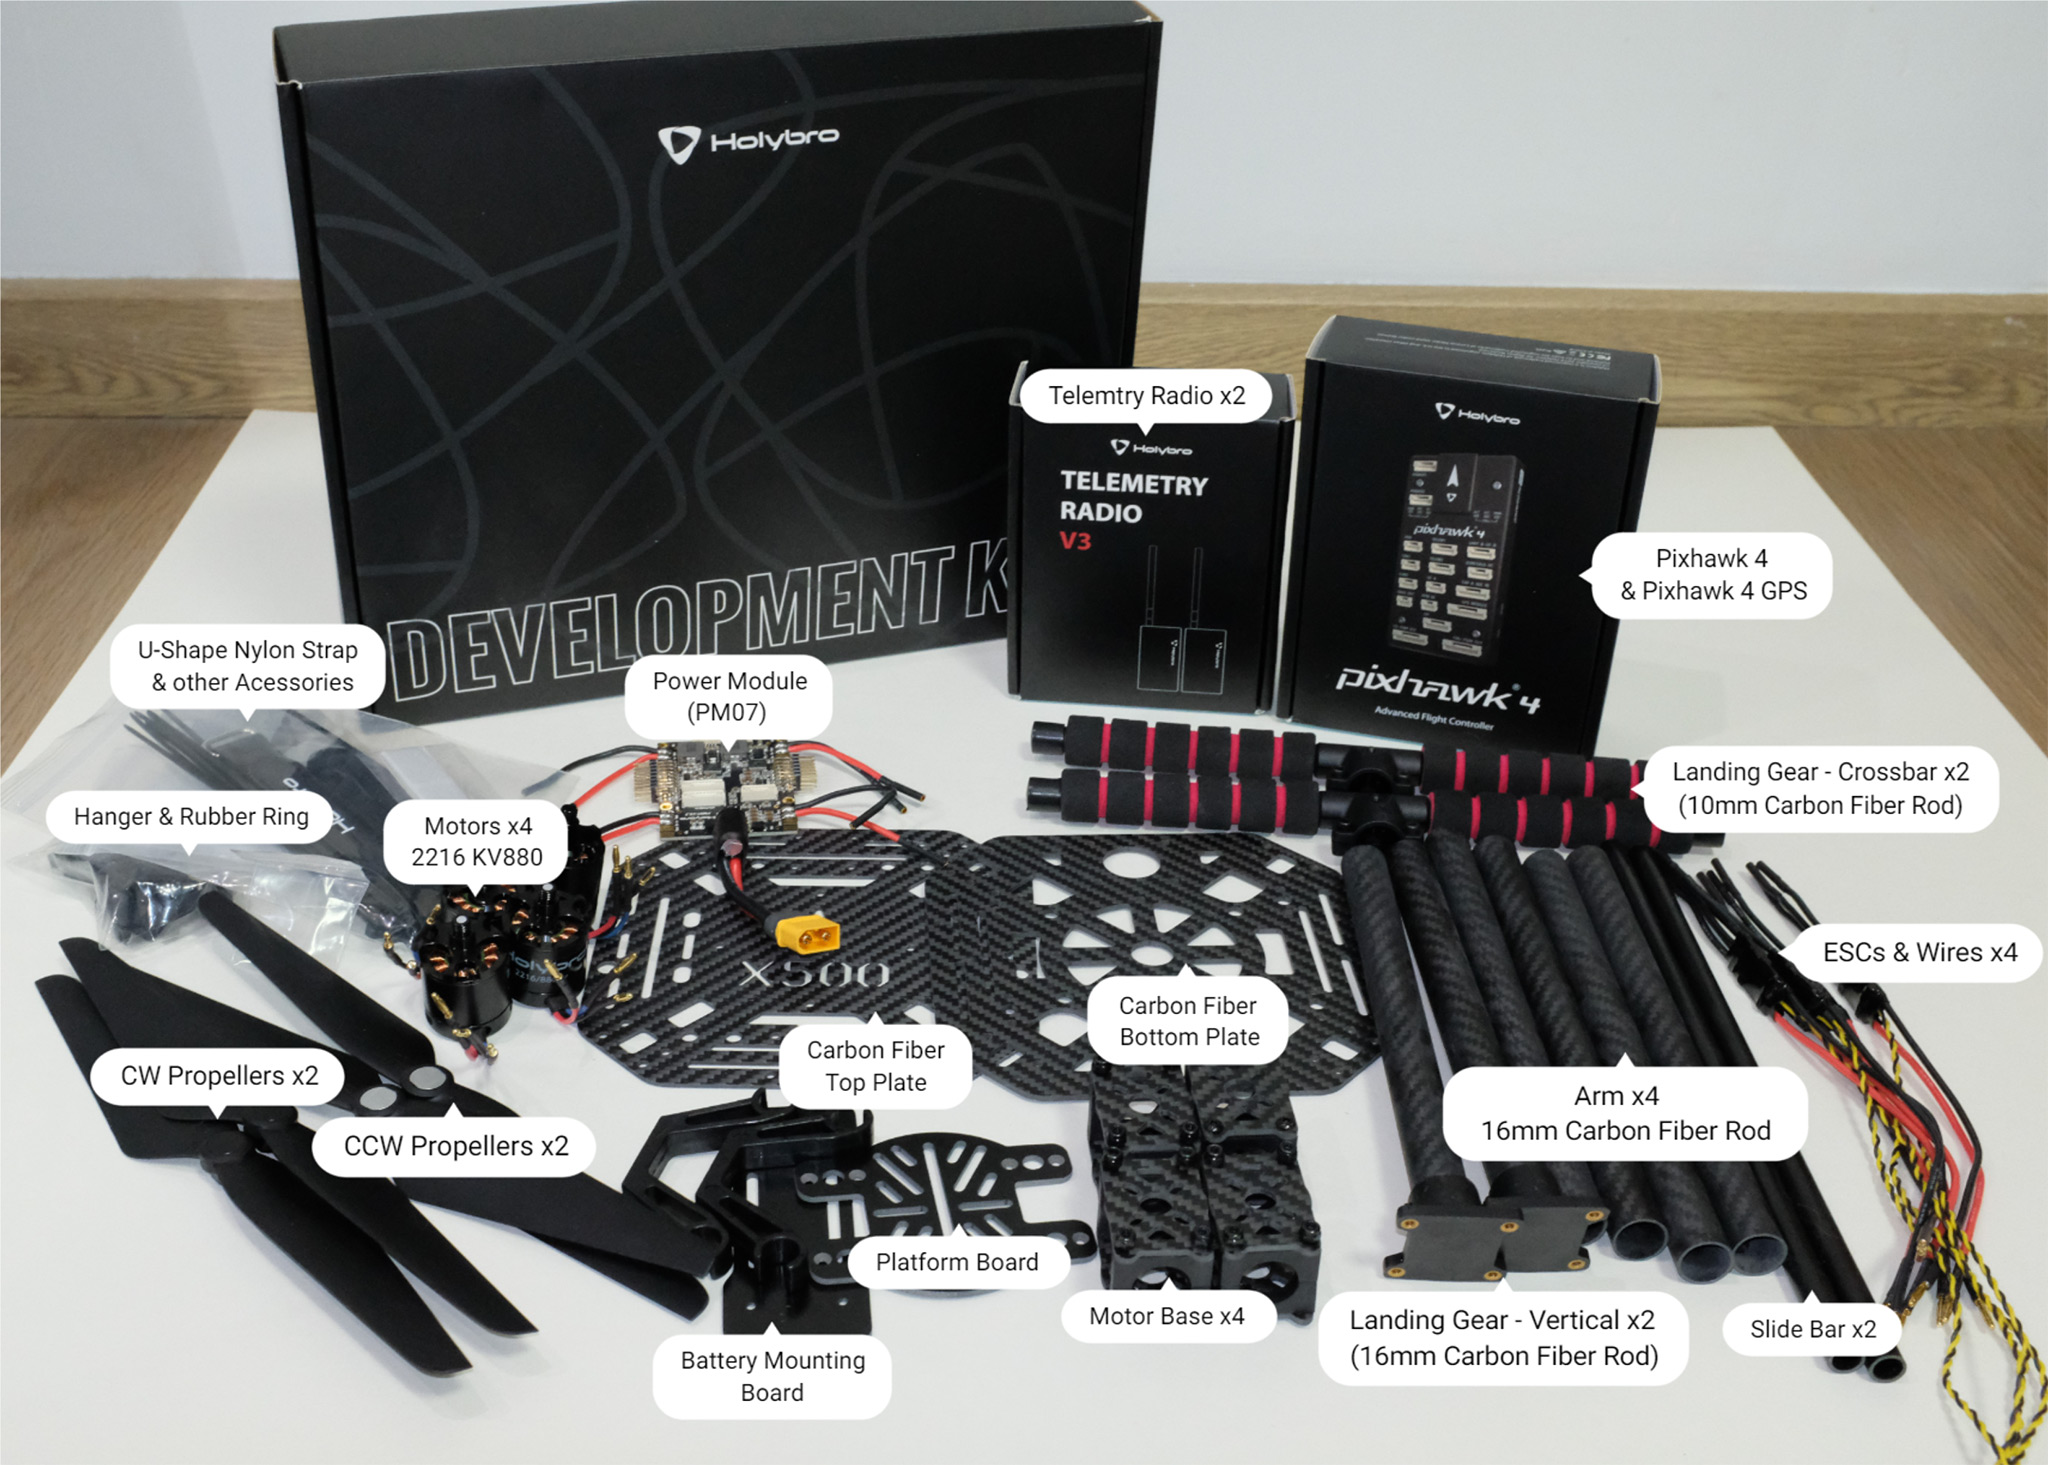
\includegraphics[width=.7\textwidth, keepaspectratio]{img/x500-dev-kit.jpg}
  \caption{Development kit for the Holybro X500.}
  \source{Adapted from \citetitle{px4-guide} \cite{px4-guide}.}
  \label{fig:x500-dev-kit}
\end{figure}


Once the standard parts are assembled, the custom additions can be integrated into the remaining space within the frame. The Raspberry Pi companion computer will be positioned between the autopilot and GPS antenna. This placement facilitates a convenient connection between the autopilot and the Raspberry Pi's I/O pins using short cables, preventing excessive wire clutter within the frame. 


\begin{figure}
  \centering
  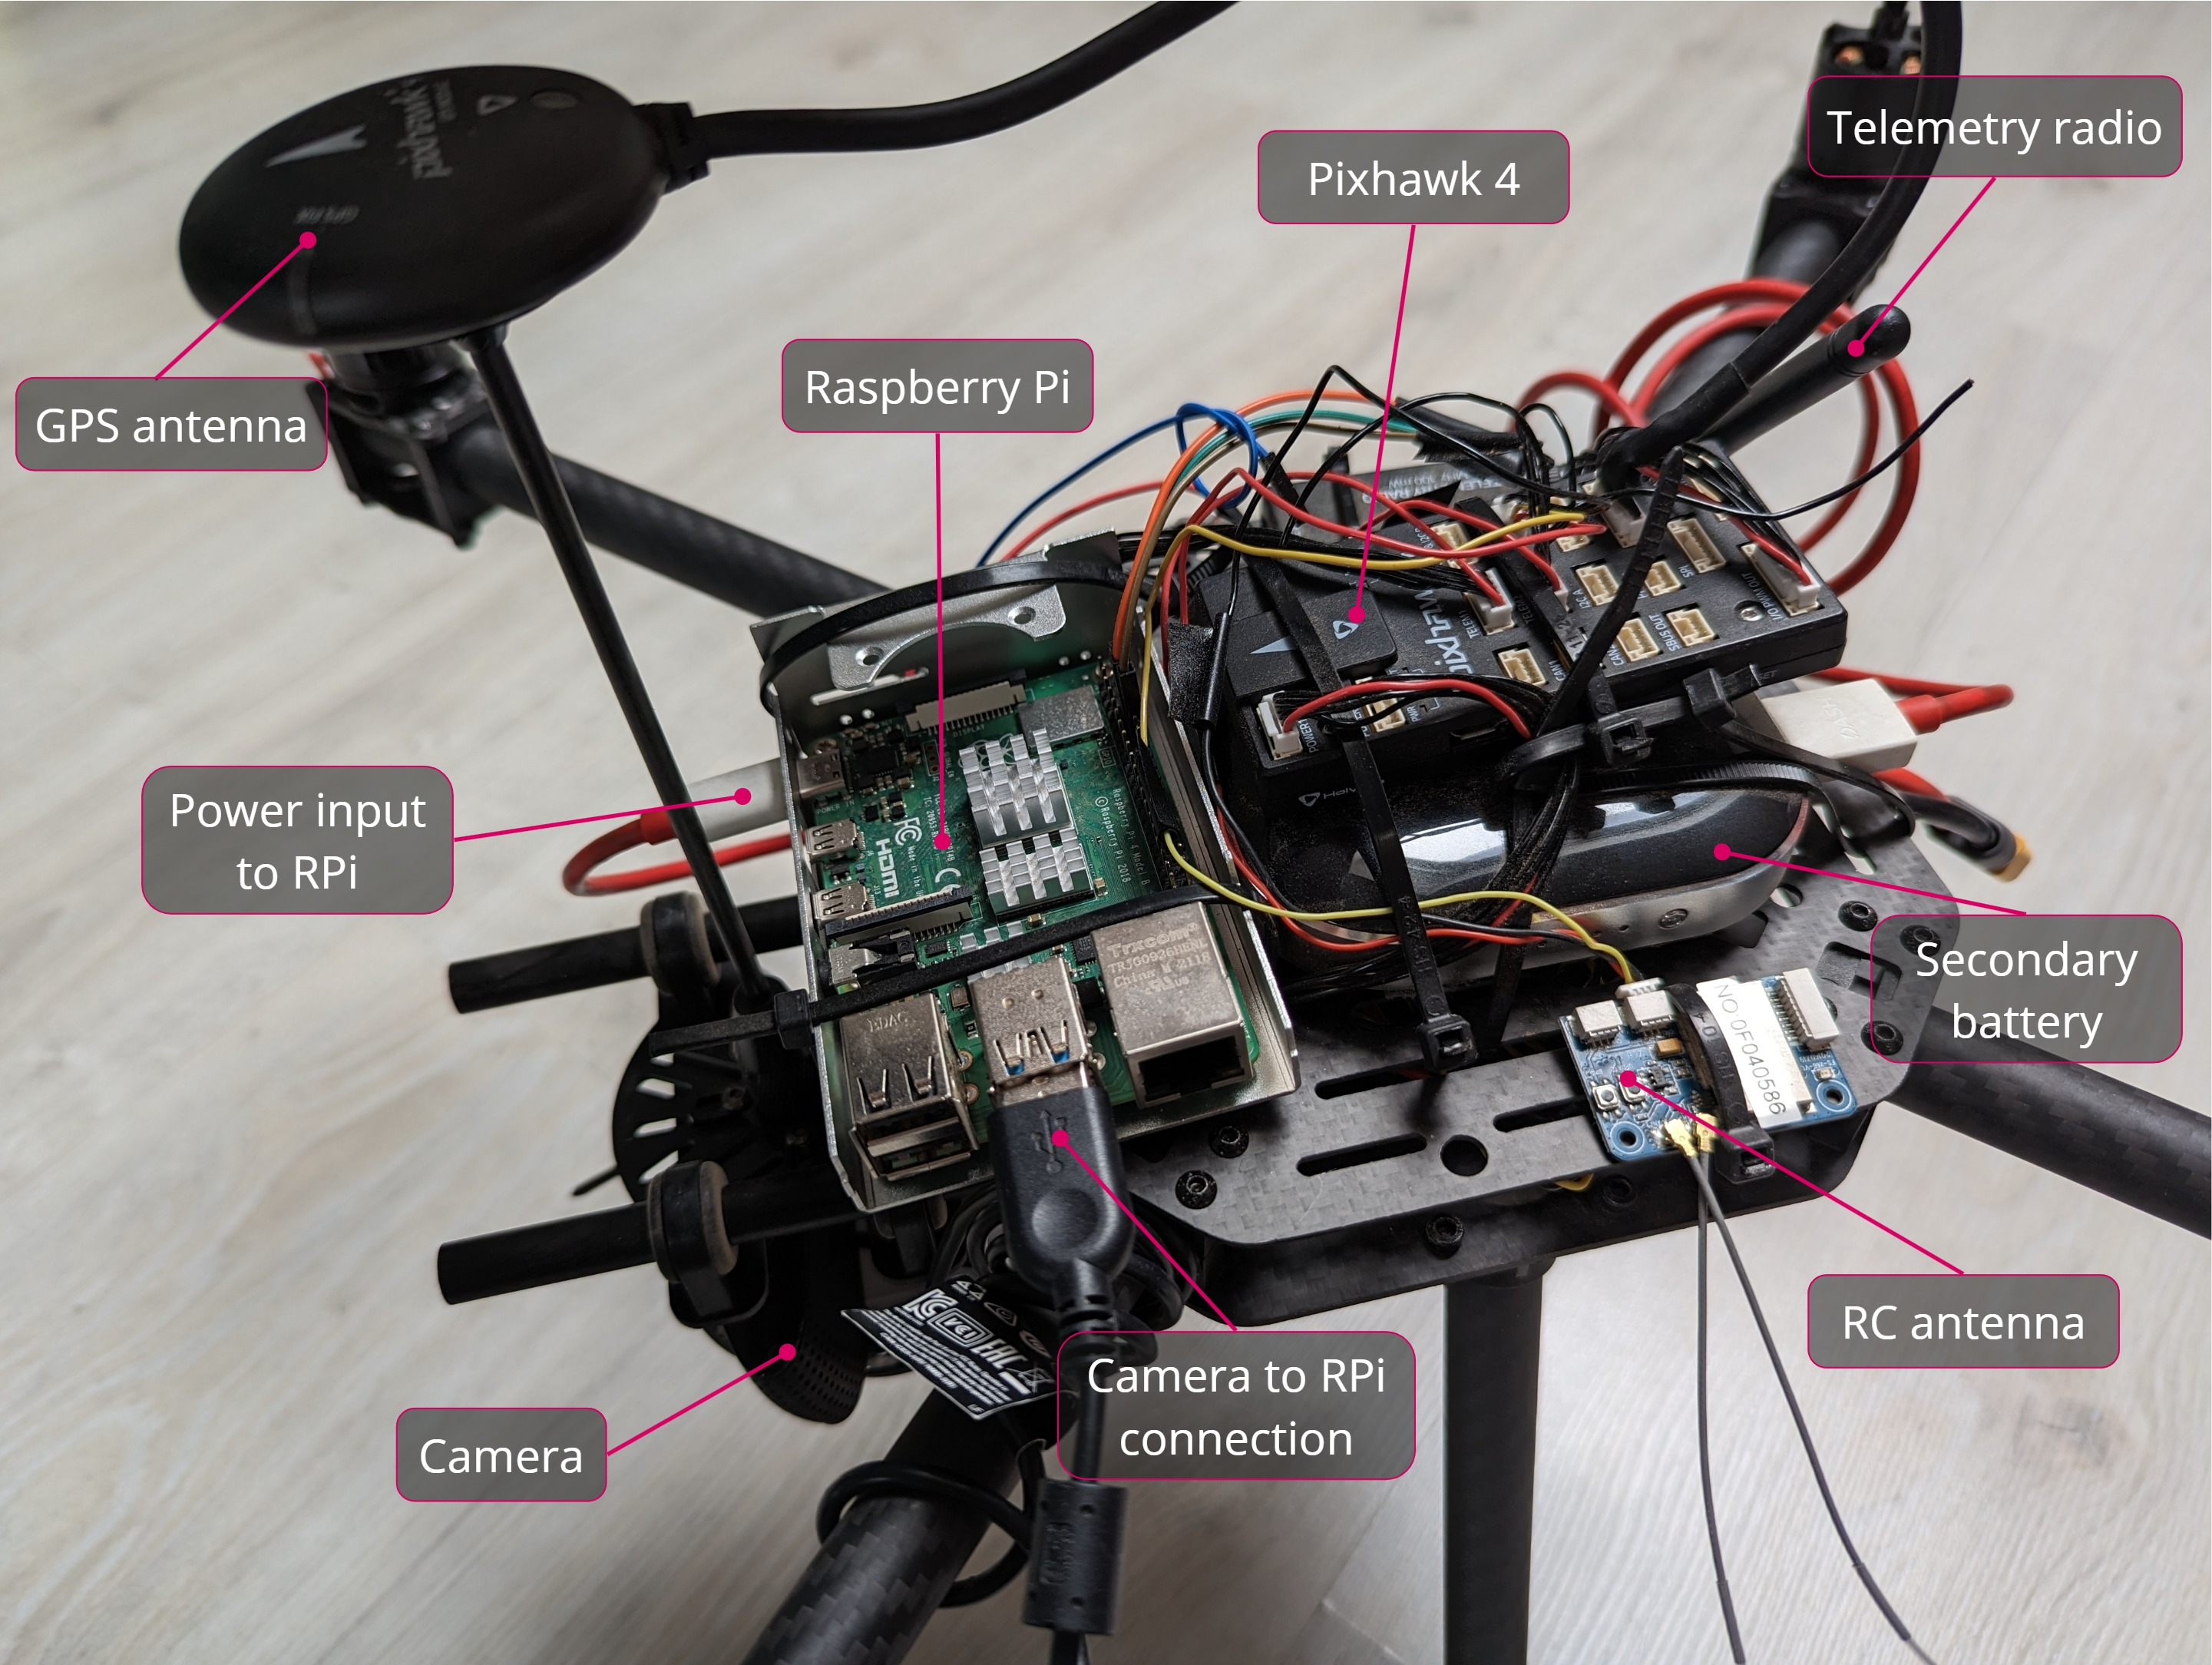
\includegraphics[width=1\textwidth, keepaspectratio]{img/full-build.jpg}
  \caption{Complete build of the quadcopter with the main components highlighted.}\label{fig:full-build}
\end{figure}

During flight, the Raspberry Pi will be powered by a dedicated external battery, which supplies power through a 2-ampere USB port. This port will be connected to the Raspberry Pi's original power cable, utilizing its USB-C power supply socket. As explained in Section \ref{sec:test-5-rpi}, this power supply is sufficient to operate the connected camera and run the developed software with satisfactory performance. The battery will be positioned beneath the autopilot, as depicted in Figure \ref{fig:full-build}. 


To ensure the camera is securely mounted on the vehicle's frame, the custom-built support system described in Section \ref{subsec:onboard} will be utilized. The camera holder will be attached to the slide bars beneath the main frame, positioning the camera's weight as close to the centre of mass as possible behind the GPS platform. The main battery, responsible for powering the engines and autopilot, and located on the underside of the carbon frame, can be shifted along the forward axis to balance the added weight from the companion computer, its battery and the camera so that the centre of gravity falls approximately in the centre of the vehicle. Figure \ref{fig:camera-holder-closeup} shows the vehicle's underside with the attached camera and the strap for holding the main battery.

\begin{figure}[H]
  \centering
  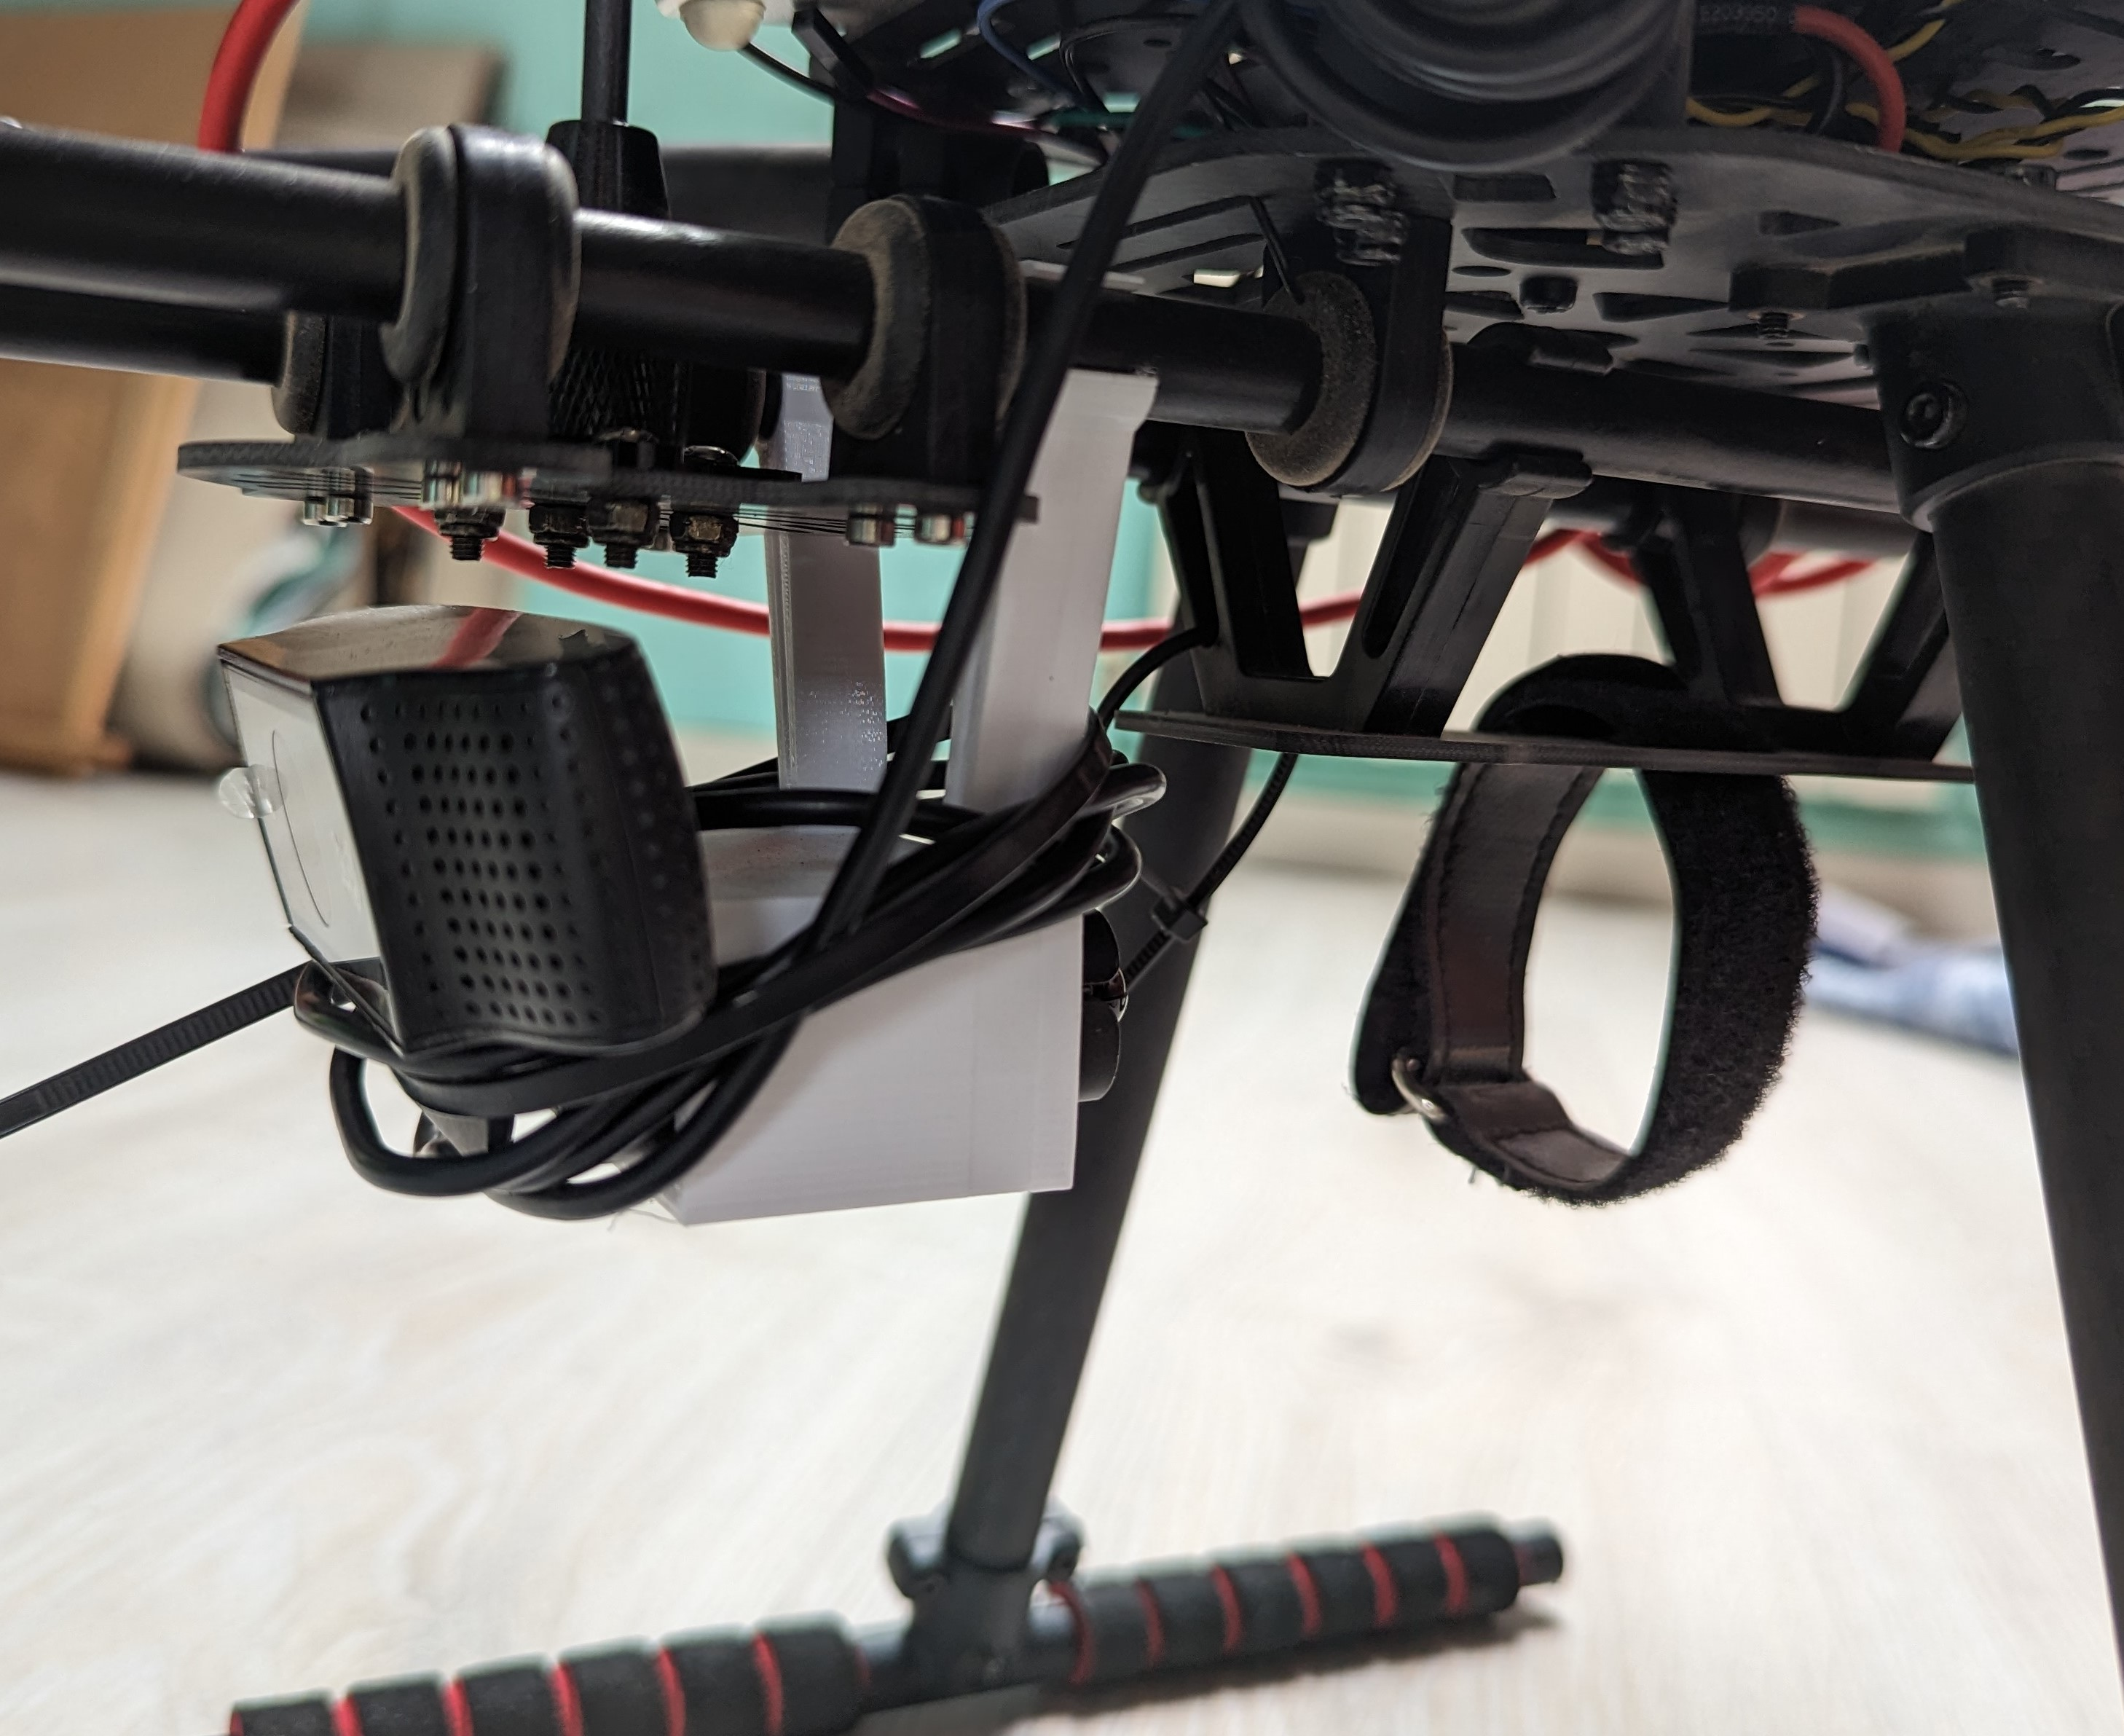
\includegraphics[width=0.6\textwidth, keepaspectratio]{img/underside-2.jpg}
  \caption{Underside of the vehicle, with the supports for holding the main battery and the camera in place.}
  \label{fig:camera-holder-closeup}
\end{figure}


Once the vehicle construction is complete, additional installation and calibration steps are necessary before it can be flown. These steps, outlined in the build instructions, should include disabling any previously activated simulation modes in the vehicle configuration. Furthermore, the \texttt{MAV\_1\_CONFIG} parameter must be set to \texttt{TELEM2}, as explained in Section \ref{subsec:offboard}. Calibration of all the onboard and externally attached sensors specific to this build is also required. The QGroundControl ground station application provides a configuration screen with the necessary calibration tools for vehicle setup, as depicted in Figure \ref{fig:qgc-config}. The vehicle configuration can be performed either by directly connecting the flight controller to a computer via the micro-USB port or wirelessly by connecting the companion telemetry radio to the computer running QGroundControl.


\begin{figure}[H]
  \centering
  \makebox[\textwidth][c]{
  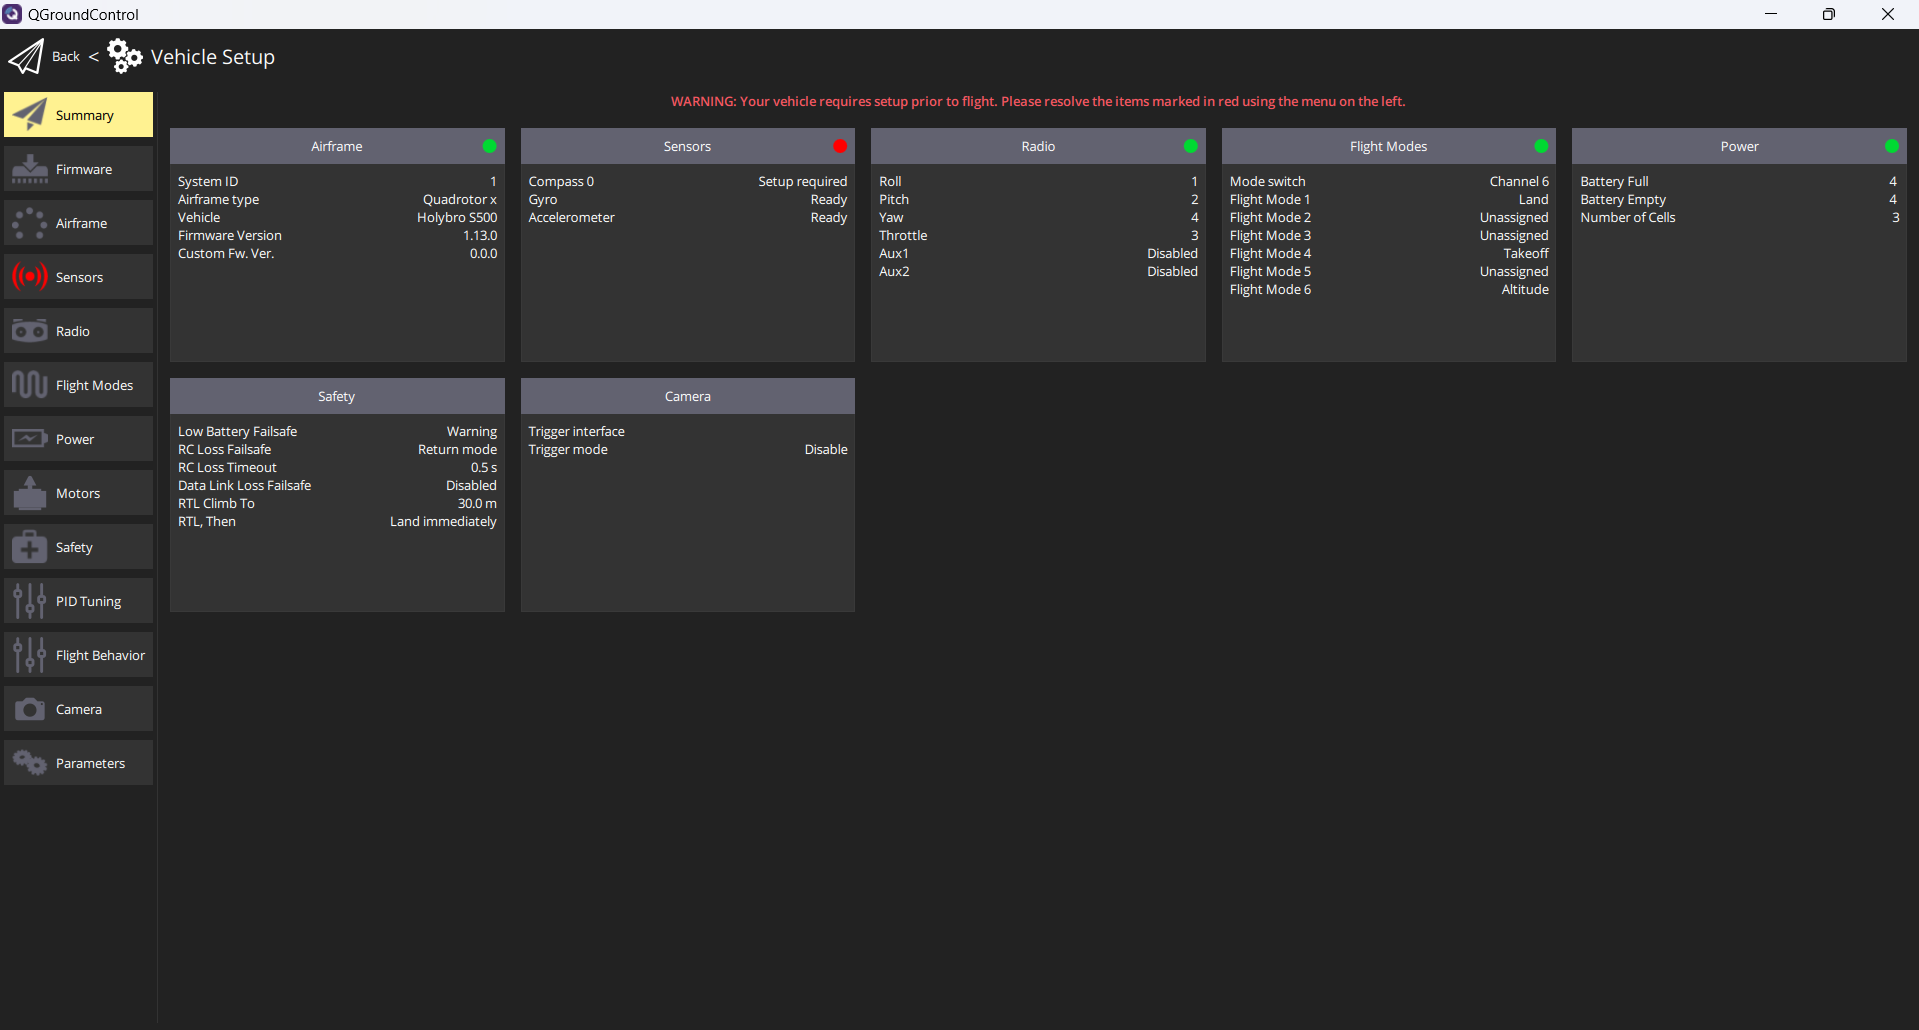
\includegraphics[width=0.5\textwidth, keepaspectratio]{img/qgc-config-1.png}
  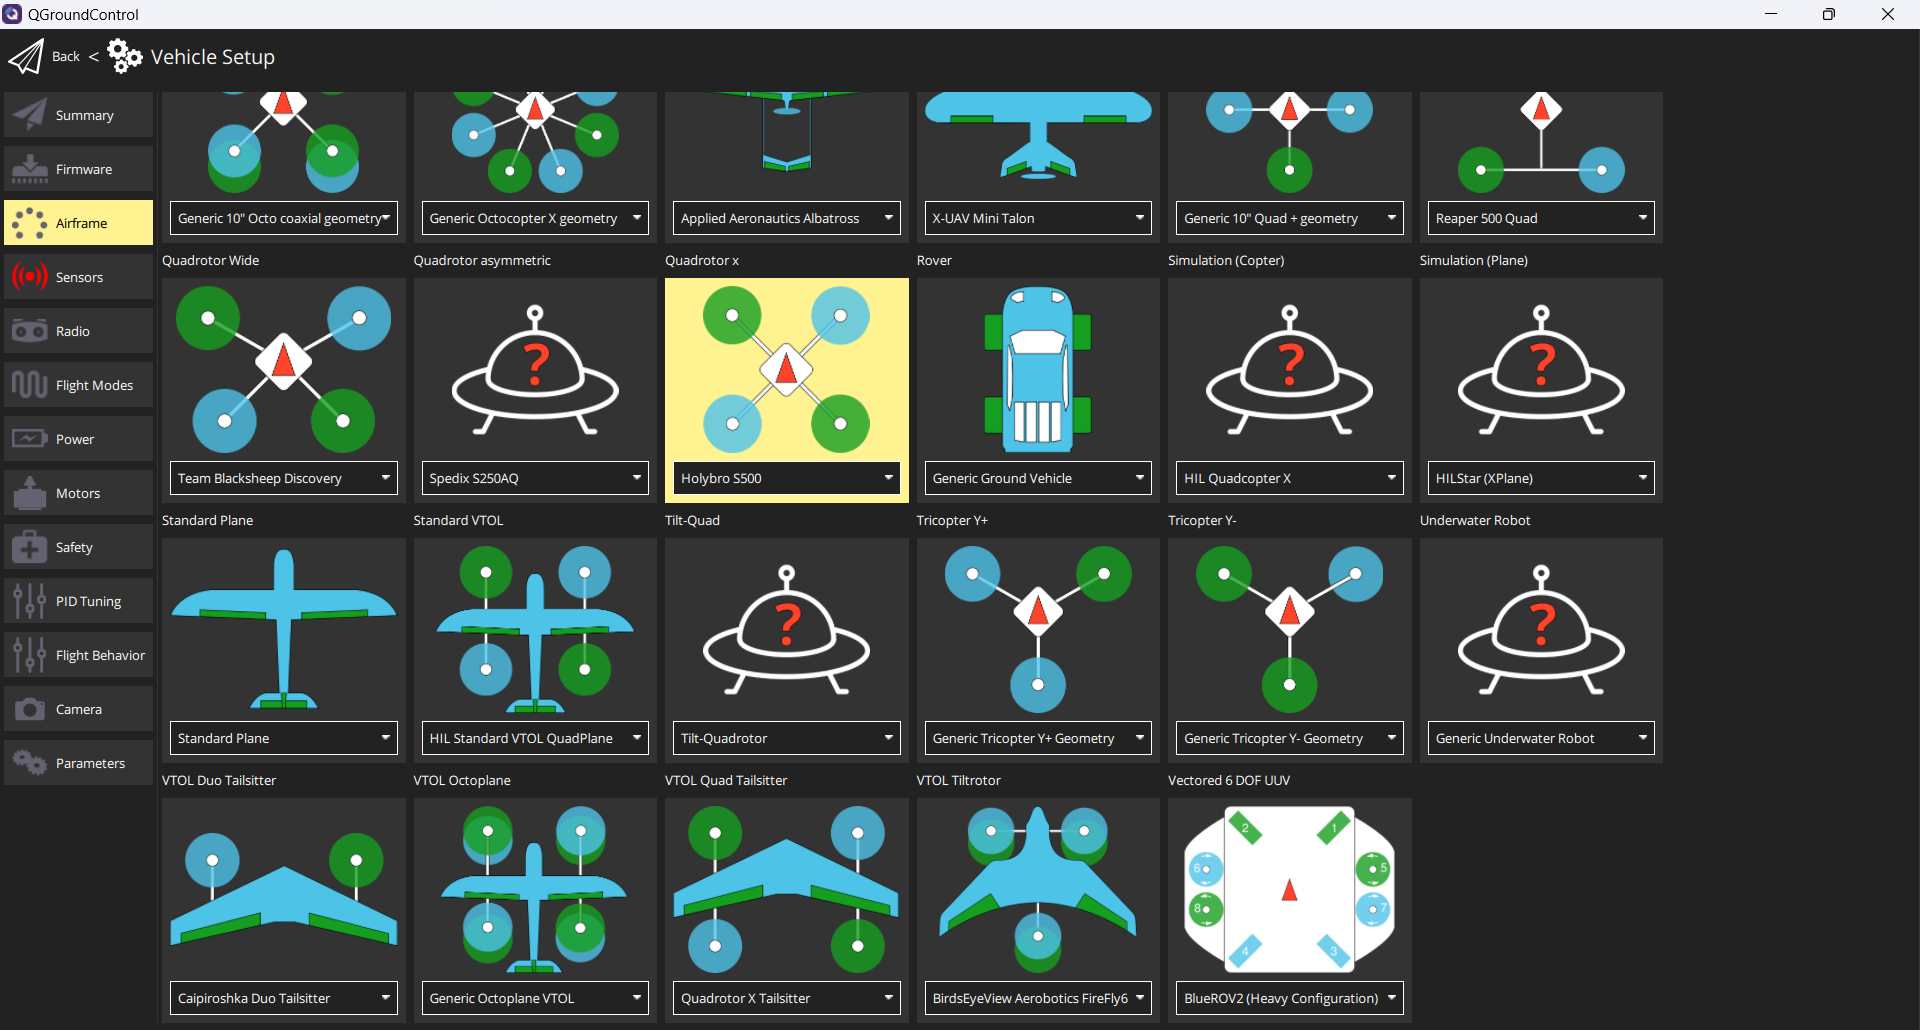
\includegraphics[width=0.5\textwidth, keepaspectratio]{img/qgc-config-3.png}}\\
  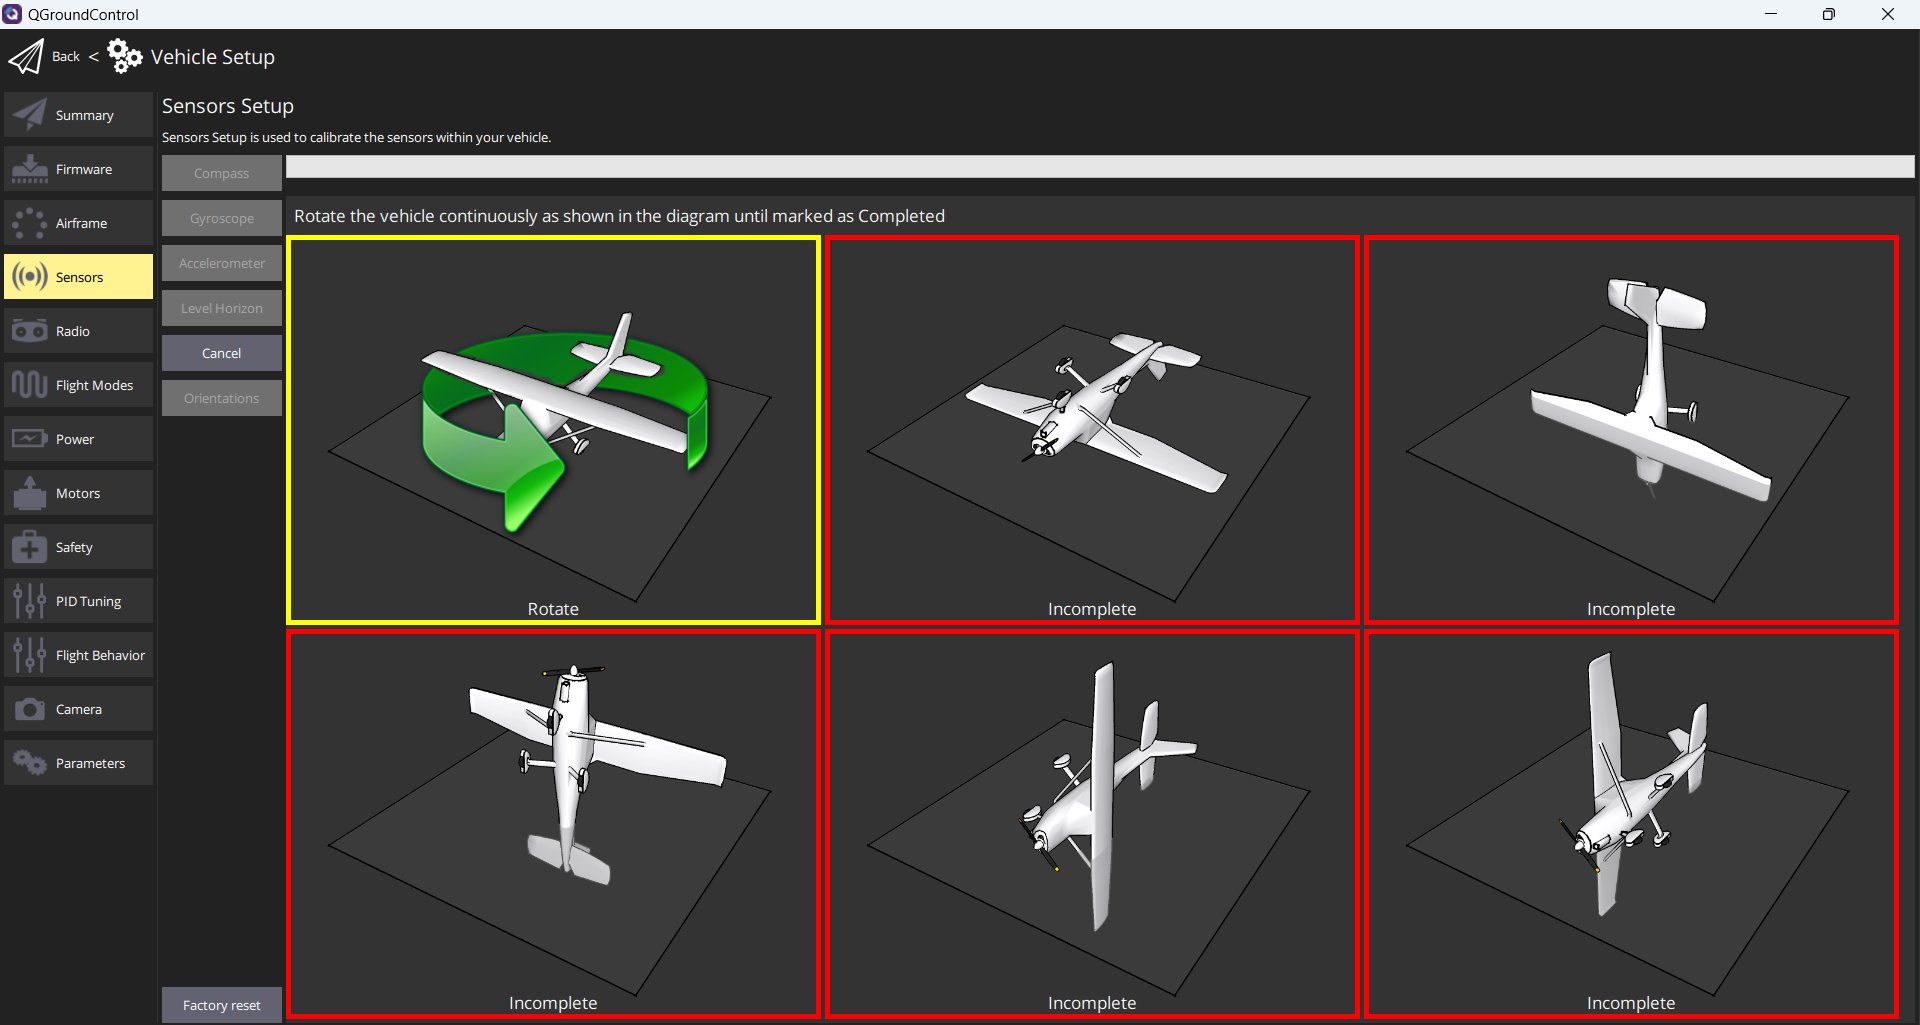
\includegraphics[width=0.5\textwidth, keepaspectratio]{img/qgc-config-2.png}
  \caption{Screenshot from the QGroundControl calibration and setup tools used to configure the vehicle}\label{fig:qgc-config}
\end{figure}


\subsection{Initial tests}
\label{sec:test-8-flight}


\subsubsection{Baseline flight with factory software}
\label{subsec:fl-test-1}

Once the vehicle is fully configured, testing the assisted takeoff and landing can be conducted using the RC controller and QGroundControl. At this stage, the drone should be capable of maintaining stable flight using autopilot-assisted flight modes, such as Position Mode. In Position Mode, the roll and pitch sticks in the controller control the vehicle's acceleration over the ground in the forward/backward and left/right directions, respectively, relative to the vehicle's heading. The throttle stick controls the ascent and descent speed. When the sticks are centred, the vehicle actively maintains its position in 3D space, compensating for wind and external forces. This semi-manual mode can serve as a safe means to verify the functionality of the factory autopilot.


Through QGroundControl, it is possible to map different switches on the RC controller to various autopilot commands. For the test, a two-position switch will be mapped to the armed/disarmed state in order to control the quadcopter's engine startup. A three-position switch will be assigned to change the vehicle's flight mode between the landing, takeoff and position modes. By shifting between the available switch positions during flight, the primary autopilot modes can be tested. Any other flight modes or triggers that need to be used can be set directly through the QGroundControl interface during flight.


To initiate the flight, the main battery is connected to the power module socket. This action powers up the autopilot, GPS antenna, telemetry radio, and RC receiver. Subsequently, QGroundControl is launched on a computer connected to the second telemetry radio via USB. If all connections have been established correctly, the ground station application will automatically connect to the vehicle and display its position on a satellite map. Similarly, turning on the RC controller establishes its connection with the vehicle, provided they have been correctly paired together as outlined in the build instructions guide. Once all wireless connections are established, the drone can take off by switching to the armed state, followed by selecting the takeoff flight mode. While the drone is airborne, switching to the position flight mode enables direct control through the joysticks on the controller.


\subsubsection{Offboard computer flight with test tool}
\label{subsec:fl-test-2}

The second test flight aims to verify that the custom software (DroneVisionControl) can wirelessly transmit takeoff and landing commands from the offboard computer using a MAVlink channel. The channel will be established by taking advantage of the developed \texttt{test-camera} tool through the telemetry radio. During this flight, it is important to note that the QGroundControl application cannot be connected to the vehicle as it will interfere with the telemetry radio channel used by the DroneVisionControl application. Consequently, the RC controller will serve as a backup in case of any issues with the software. The controller can be used to switch flight modes and override inputs from the DroneVisionControl application, providing manual control if necessary.

Since the DroneVisionControl application will arm the vehicle on its own by sending a takeoff command and to ensure safety during flight, the two-way switch on the controller will be mapped on all subsequent tests to the command to cut off power to the engines. This command can be valuable in exceptional situations where it is necessary to protect the vehicle or the surrounding area, such as if the autopilot were to destabilize during takeoff and landing or there was a complete loss of control during flight.

To initiate the test, the main battery is reconnected to the power module. Then, the following command is executed on the offboard computer, depending on whether it is desired to be run on a Windows or Linux machine.


\begin{minted}[escapeinside=||,breaklines,fontsize=\footnotesize, baselinestretch=1]{bash}
|Windows:| dronevisioncontrol tools test-camera -r COM<X>:57600
|Linux:| dronevisioncontrol tools test-camera -r /dev/ttyUSB0:57600}
\end{minted}


After successfully establishing the connection with the vehicle, the computer keyboard can be used to control the flight. Pressing the T key triggers takeoff, while the L key initiates the landing process. The O key sets the autopilot to offboard flight mode, enabling it to receive velocity commands. Subsequently, the WASD keys will control the forward and sideways movement of the vehicle, and the QE keys will adjust its yaw rotation.

Figure \ref{fig:flight-test-cam-offboard} illustrates the output displayed in the computer's terminal window, showcasing the connection process, the sent velocity commands, and the camera output from the offboard computer. Additionally, a video capturing the entire process can be accessed in the project's href{https://l-gonz.github.io/tfg-giaa-dronecontrol/videos/flight-test-offboard}{website}\footnote{\url{https://l-gonz.github.io/tfg-giaa-dronecontrol/videos/flight-test-offboard}}.

\begin{figure}
  \centering
  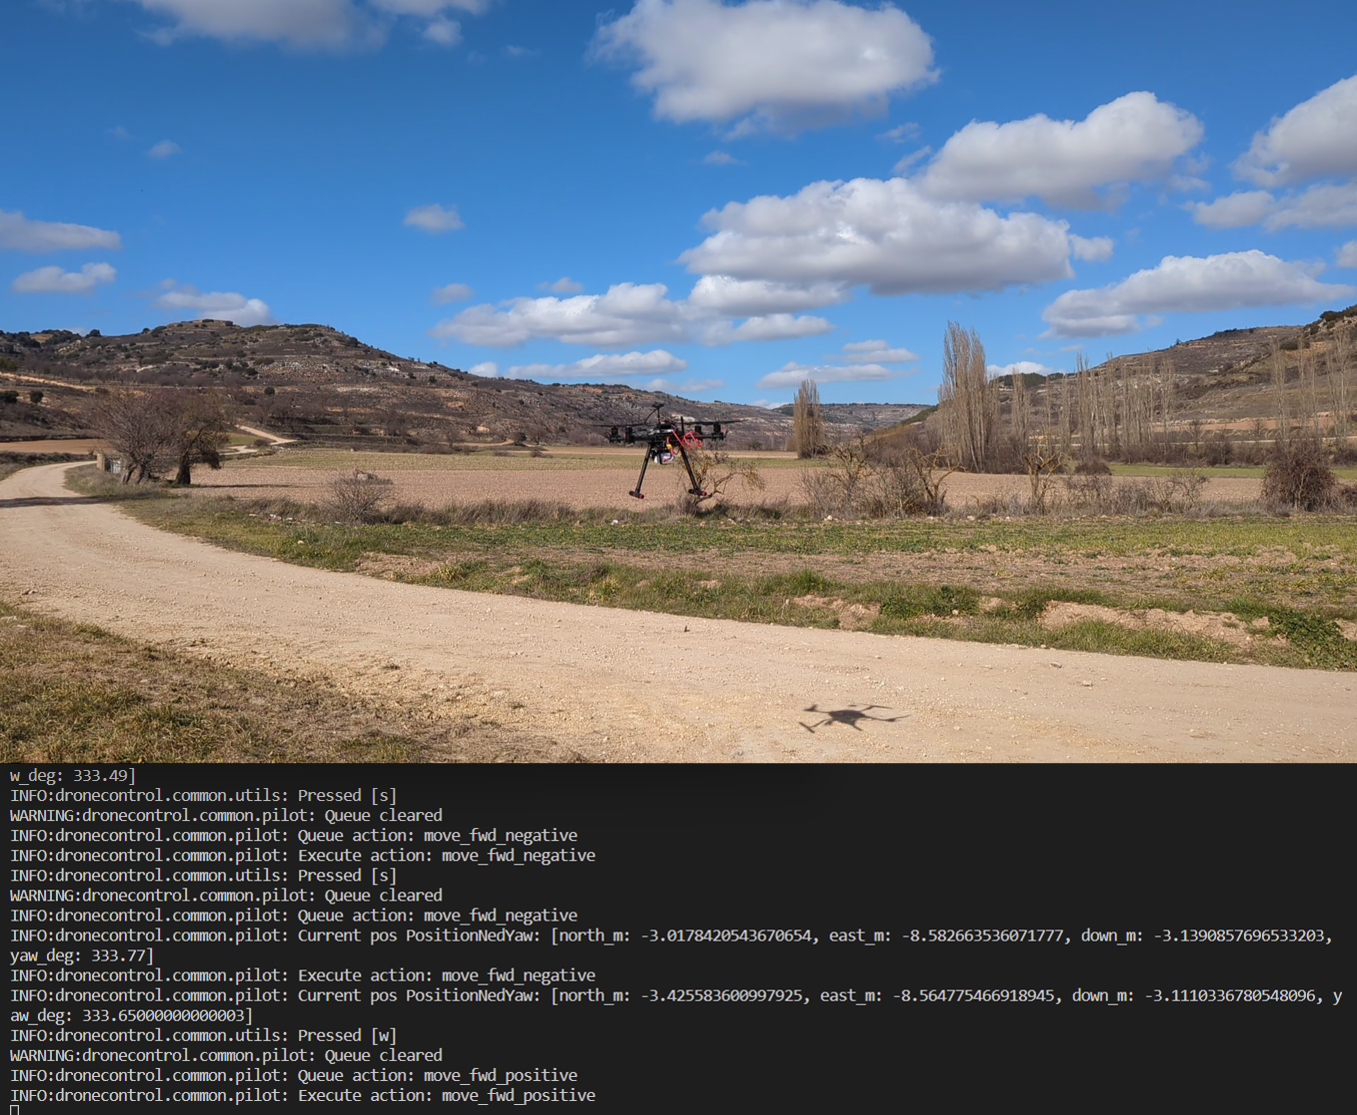
\includegraphics[width=\textwidth, keepaspectratio]{img/video-field-test-offboard.png}
  \caption{Terminal output from the \texttt{test-camera} tool running on an offboard computer and image of the drone flying in response}
  \label{fig:flight-test-cam-offboard}
\end{figure}

\subsubsection{Onboard computer flight with test tool}
\label{subsec:fl-test-3}


The third and final test flight in this section aims to confirm that the custom software can send takeoff and landing commands through a cabled MAVlink channel from the onboard computer. Additionally, it ensures that the onboard camera can capture a clear image of the vehicle's field of view during flight.

For this test, the same tool used in the previous test will be executed on the Raspberry Pi, utilizing the wired serial link between the onboard computer and the Pixhawk autopilot board. As the tool will now use the camera connected to the companion computer, positioned to look down on the pilot, pose detection can be activated on the received images.


To initiate the flight test, the main battery needs to be attached to the power module and the secondary battery to the Raspberry Pi. Once the onboard computer has started, it will be operated through a remote desktop connection via WiFi. Using this connection, a terminal window can be opened on the desktop to execute the following command:
\begin{minted}[breaklines, fontsize=\footnotesize, baselinestretch=1]{bash}
dronevisioncontrol tools test-camera -r /dev/serial0:921600 -p
\end{minted}


Unlike the telemetry radio flight, this test employs a serial connection running at a baud rate of 921600, matching the configured baud rate on the \texttt{TELEM2} port of the Pixhawk board. The \texttt{-p} option enables pose detection in the output images. A video documenting the entire process can be accessed on this \href{https://l-gonz.github.io/tfg-giaa-dronecontrol/videos/flight-test-onboard}{link}\footnote{\url{https://l-gonz.github.io/tfg-giaa-dronecontrol/videos/flight-test-onboard}}. Additionally, an image extracted from the video can be seen in Figure \ref{fig:flight-test-cam-onboard}.


\begin{figure}
  \centering
  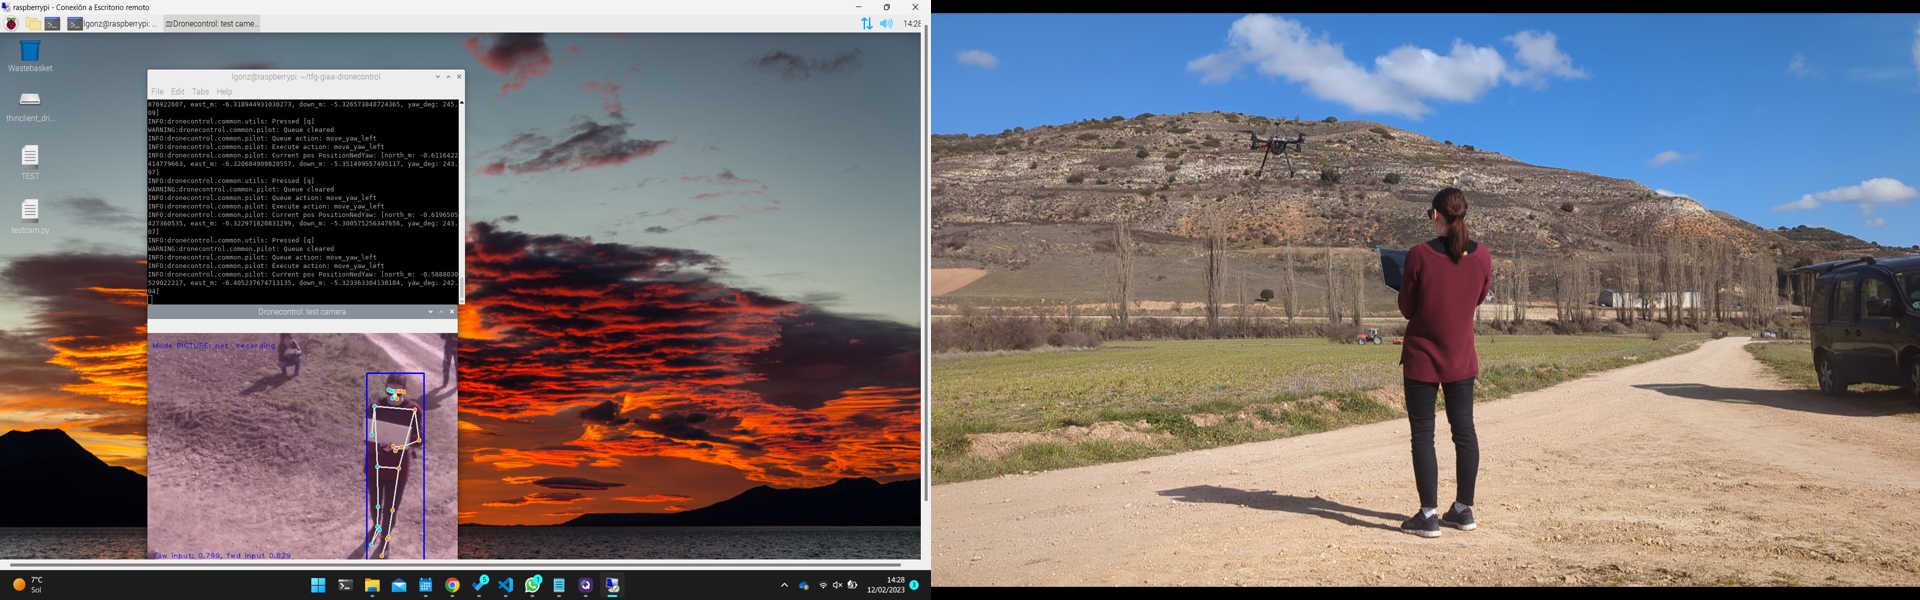
\includegraphics[width=\textwidth, keepaspectratio]{img/video-field-test-onboard.png}
  \caption{Pose detection algorithm running on images taken during flight}
  \label{fig:flight-test-cam-onboard}
\end{figure}


\subsection{Hand gesture control}
\label{subsec:fl-test-4}


During the basic flight tests, all the connections and individual components of the software were validated in realistic flight scenarios. Now, the focus shifts to integrating the piloting system with the results of image recognition to test the developed vision-based control solutions.

The first solution to be tested in flight is the hand-gesture guidance system, which runs on an offboard computer without performance constraints and doesn't rely on battery power. The setup for this test will be the same as the second test flight, described in Section \ref{subsec:fl-test-2}, using the telemetry radio for the serial link and disregarding the onboard companion computer. Once the autopilot board is powered up, the control solution is initiated by executing the following command, where <device> is replaced with the appropriate COM port or TTY device to which the telemetry radio is connected, depending on the platform.
\begin{minted}[breaklines, fontsize=\footnotesize, baselinestretch=1]{bash}
dronevisioncontrol hand -s <device>:57600
\end{minted}


Once the pilot connection is established, the image from the computer's webcam will be displayed on the screen with an outline highlighting any detected hand. To begin controlling the vehicle, the open palm gesture should be shown to the camera. Closing the hand into a fist will initiate takeoff, and pointing up with the index finger will activate the offboard flight mode. Moving the index finger right or left will cause the vehicle to mirror the movement, while moving the thumb right or left will make the vehicle move forwards and backwards, respectively. At any point during the test, displaying an open hand will cause the drone to hover in its current position. Losing sight of the controlling hand will also trigger the hovering mode.


A video showcasing the entire process can be accessed on this \href{https://l-gonz.github.io/tfg-giaa-dronecontrol/videos/flight-test-hand}{link}\footnote{\url{https://l-gonz.github.io/tfg-giaa-dronecontrol/videos/flight-test-hand}}. Additionally, an image extracted from the video can be seen in Figure \ref{fig:flight-test-hand}.

\begin{figure}
  \centering
  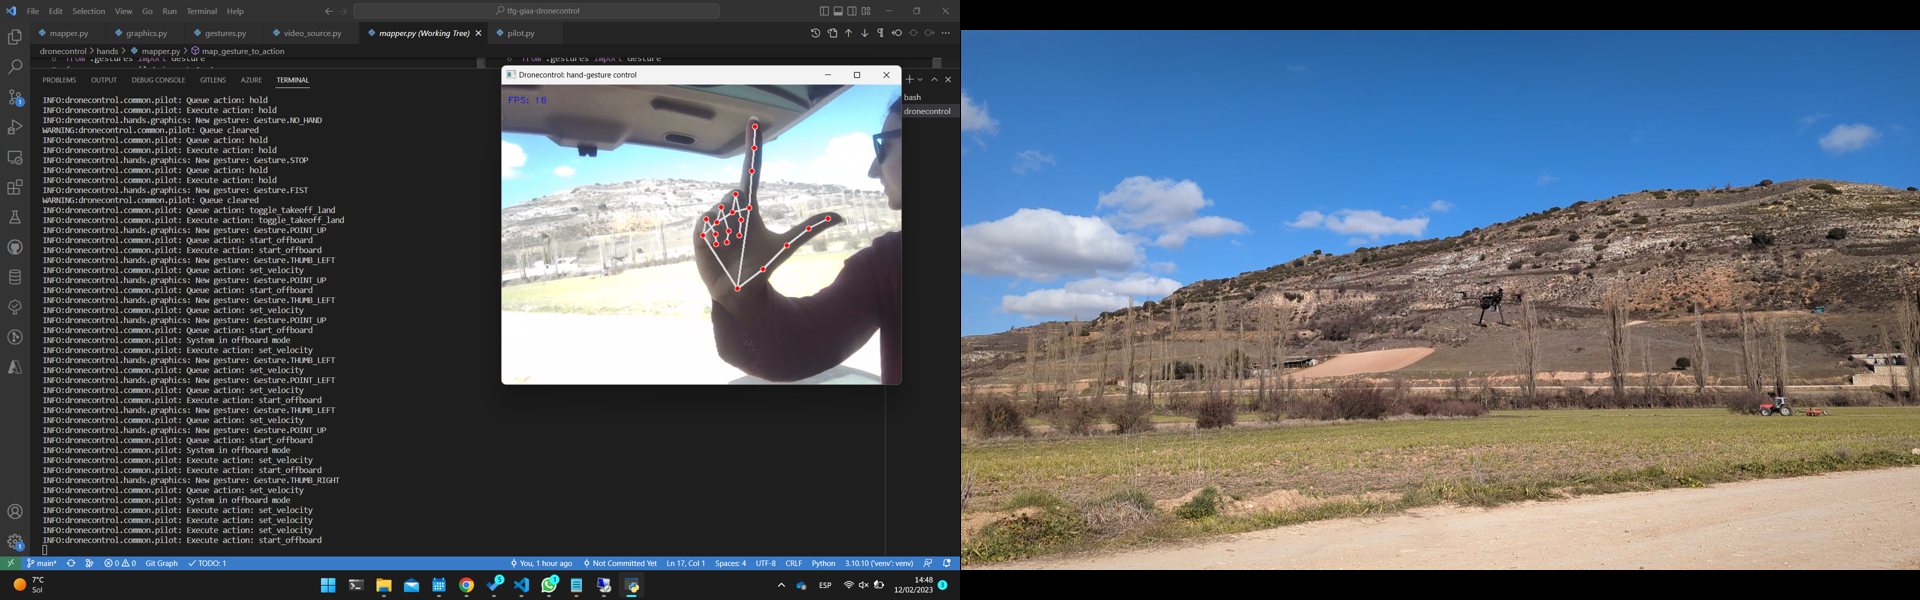
\includegraphics[width=\textwidth, keepaspectratio]{img/video-field-test-hand.png}
  \caption{Image taken during flight controlled by the hand-gesture solution. The vehicle is moving forward.}
  \label{fig:flight-test-hand}
\end{figure}


\subsection{Target detecting, tracking and following}
\label{subsec:fl-test-5}

The last test to conduct is for the follow control solution. In this section, the companion computer will run the follow program with the aim of tracking and following a moving target outside of simulation. The setup for this test will be the same as the third test flight, described in Section \ref{subsec:fl-test-3}. Without the need for a wireless telemetry connection on the DroneVisionControl side, the telemetry radio can be utilized to track the vehicle's path using the QGroundControl application on a secondary offboard computer. The control application will be started with the following command:
\begin{minted}[breaklines, fontsize=\footnotesize, baselinestretch=1]{bash}
dronevisioncontrol follow -s /dev/serial0:921600
\end{minted}
This \href{https://l-gonz.github.io/tfg-giaa-dronecontrol/videos/flight-test-follow}{video}\footnote{\url{https://l-gonz.github.io/tfg-giaa-dronecontrol/videos/flight-test-follow}} showcases the process of the vehicle taking off (T key) and activating offboard flight mode (O key) to initiate the tracking of a detected figure. Figure \ref{fig:flight-test-follow} presents an image extracted from this video.


\begin{figure}
  \centering
  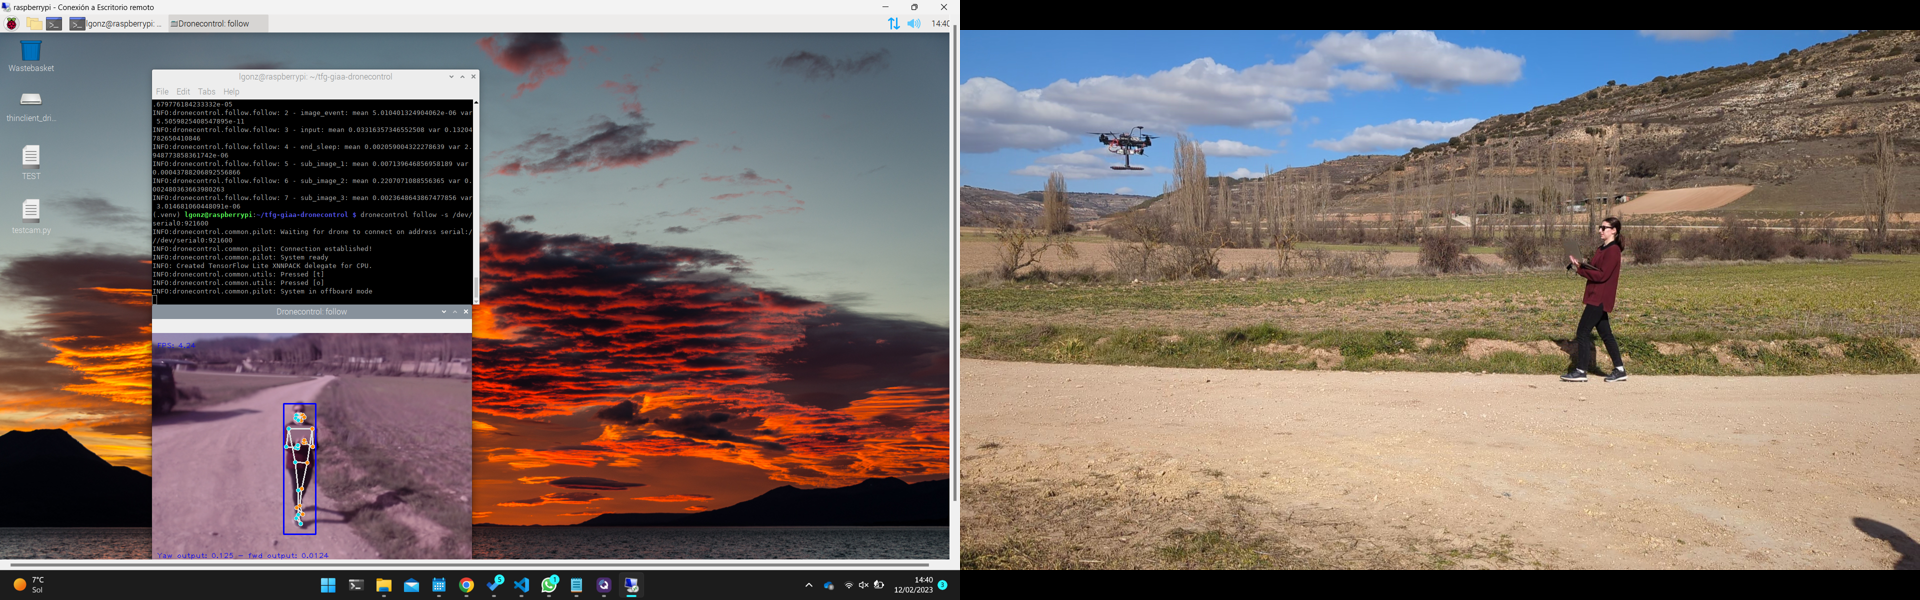
\includegraphics[width=\textwidth, keepaspectratio]{img/video-field-test-follow.png}
  \caption{Terminal and image output of the DroneVisionControl follow solution running on the Raspberry Pi}
  \label{fig:flight-test-follow}
\end{figure}


During the flight test, the application running on the Raspberry Pi achieves a maximum frame rate of around 6 FPS when the follow mechanism is active and approximately 8 FPS when it is disabled by switching out of offboard flight mode. In practical terms, this means that the person being tracked by the drone needs to move relatively slowly to ensure that the camera does not lose sight of them before the control loop can send the command to the vehicle to move to the previously detected position. However, for a proof-of-concept scenario, this performance is acceptable.


At the end of the program execution, the average loop time and average runtime for each task in the control loop are displayed in the terminal. Based on the measurements obtained during the test flight, the average frame rate is calculated to be 3.58 FPS. Figure \ref{fig:flight-performance} compares these measurements with those analyzed in Section \ref{subsec:performance}, particularly with the test configuration selected to most closely resemble actual flight conditions (autopilot board running on HITL mode and the companion computer powered by the secondary battery). Very similar results are recorded for both tests, confirming the simulation configuration employed as a valid method of obtaining realistic results without complex or costly flight tests.

Overall, this test flight verifies the effectiveness of the follow control solution and its ability to track and follow a moving target during a real flight scenario, as well as the validity of the simulation process to obtain realistic results.

\todo[inline]{Are frame rates swapped on graphs ????}

\begin{figure}
  \centering
  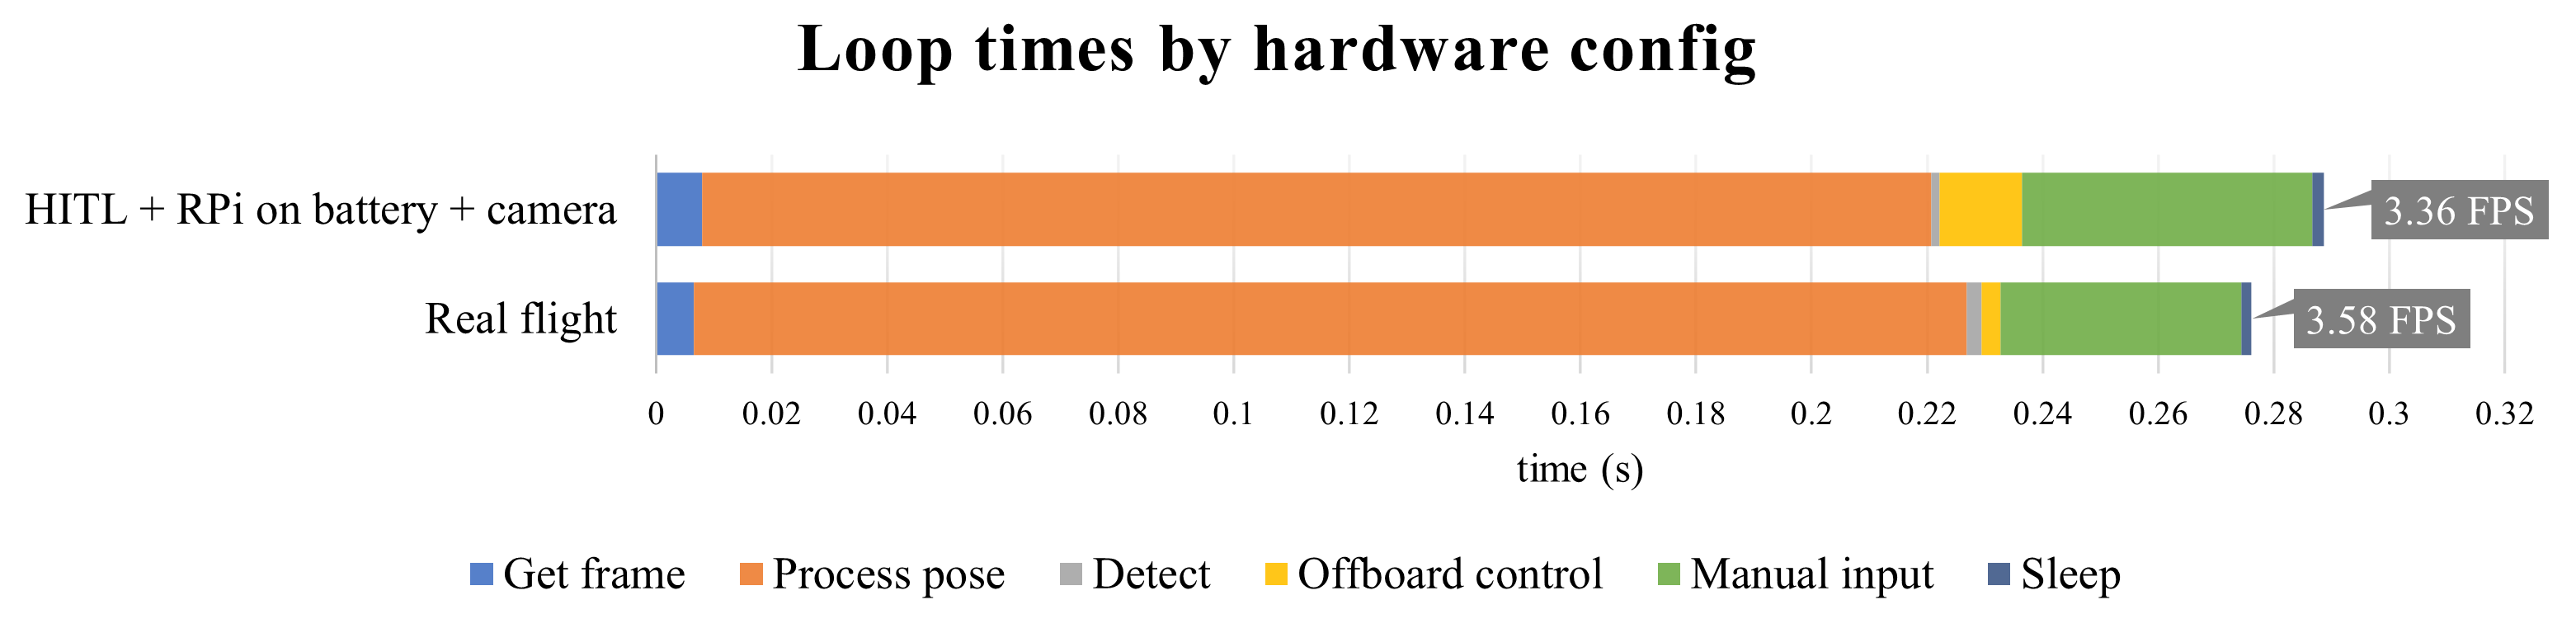
\includegraphics[width=\textwidth, keepaspectratio]{img/perf-hitl-flight.png}
  \caption{Average loop time for each individual task in the follow control solution and total frame rate for realistic simulation versus actual test flights.}
  \label{fig:flight-performance}
\end{figure}
